\chapter*{Геометрия}
\addcontentsline{toc}{chapter}{Геометрия}

\setlength{\epigraphwidth}{.72\textwidth}
\epigraph{Уравнения --- просто скучная часть математики.\\
Я пытаюсь смотреть на мир с точки зрения геометрии.}{---Стивен Хокинг (1942---2018)}

Классическая геометрия в двух- или трёхмерном пространстве является, безусловно, неисчерпаемым источником для составителей задач. 
Но нас интересуют головоломки, а это не те задачи, которые бы Евклид включил в свой Том II.
Вас не будут просить доказать, что $AB=CD$, или что один треугольник конгруэнтен другому.

Но к счастью, существует огромное множество очаровательных геометрических задач, отвечающих нашей цели. 
Задача, которую мы разберём в качестве примера, появилась в 1980 году на подготовительном  школьном экзамене, %(Preliminary Scholastic Aptitude Exam),
где, к стыду составителей из экзаменационного комитета,  
утверждённый правильным ответ оказался неверен.
И один смелый ученик, получив результат экзамена, обратился в комитет с аппеляцией.
К нашей большой радости, правильное решение являет собой  чудесное интуитивное доказательство.
(Хочу заметить, что впоследствии был создана специальная группа, в которой  трудился и ваш автор, для анализа экзаменационных заданий по математике.)

\subsection*{Склеивание пирамид}% (GLUING PIRAMIDS)
\rindex{Склеивание пирамид}

Пирамида с квадратным основанием, имеющая рёбра единичной длины, и пирамида с треугольным основанием (тетраэдр), также с рёбрами единичной длины, склеены вместе по треугольным граням.

Сколько граней имеет полученный многогранник?

\paragraph{Решение:}

Пирамида с квадратным основанием имеет пять граней, тетраэдр --- четыре.
Так как две грани склеены вместе, у получившегося многогранника будет $7=4+5-2$ граней, правильно?
Это, очевидно, была предполагаемая линия рассуждений.
Составителю задачи могло бы прийти в голову, что, в принципе, пара прилегающих граней из разных многогранников, может в после склейки оказаться в одной плоскости.
Таким образом, они сольются в одну грань, что уменьшит ответ.
Но, несомненно, такое совпадение должно быть исключено.
Ведь эти два многогранника даже не одинаковой формы.

Но на самом деле, так и случается (дважды):
склеенный многогранник имеет пять граней.
Можно вообразить себе такую картину: две пирамиды с квадратным основанием стоят на столе основаниями вниз и примыкают друг к другу по ребру основания.
Теперь, соединив вершины пирамид воображаемой линией, отметим, что длина полученного отрезка равна единице, как и все рёбра пирамиды.

Таким образом, между двумя пирамидами с квадратным основанием помещается правильный тетраэдр.
Две плоскости, каждая из которых содержит по треугольной грани от каждой из двух пирамид, также содержит и грань тетраэдра.
Отсюда результат.
\heart

(Если это сложно представить, посмотрите картинку ниже.)

Данное доказательство, иногда называемое «палаточным решением», появилось в 1982 в статье Стивена Янга.%
\footnote{S. Young, ``The mental representation of geometrical knowledge''. \emph{The Journal of Mathematical Behavior} (1982).}

\begin{figure}[h!]
\centering
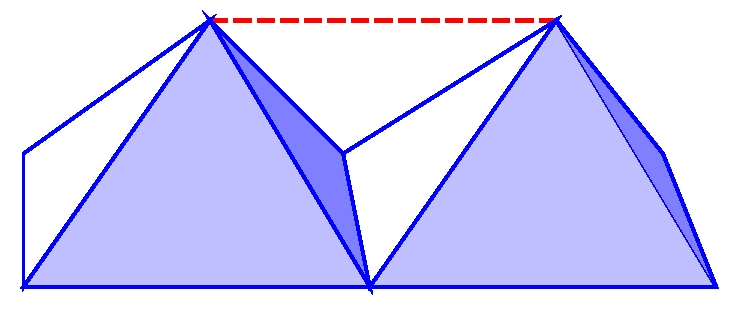
\includegraphics[scale=0.55]{Figs/Geometry/pyrs}
\end{figure} 

Одна из задач, приведённых ниже, имеет «доказательство без слов» --- достаточно одного рисунка.
Посмотрим, сможете ли вы догадаться, которая.

\subsection*{Окружности в пространстве}% (CIRCLES IN SPACE)
\rindex{Окружности в пространстве}

Возможно ли трёхмерное пространство разбить на окружности? 

\subsection*{Магия кубов}% (MAGIC WITH CUBES)
\rindex{Магия кубов}

Можно ли протащить куб сквозь отверстие в кубе меньшего размера?

\subsection*{Красные и синие точки}% (RED POINTS AND BLUE POINTS)
\rindex{Красные и синие точки}

На плоскости дано $n$ красных и $n$ синих точек, при этом никакие три точки не лежат на одной прямой.
Докажите, что их можно разбить на пары таким образом, что отрезки, соединяющие каждую красную точку с соответствующей ей синей, не пересекаются.

\subsection*{Прямая через две точки}% (LINE THROUGH TWO POINTS)
\rindex{Прямая через две точки}

Пусть $X$ --- конечное множество точек на плоскости, не все из которых лежат на одной прямой.
Докажите, что существует прямая, проходящая ровно через две точки из $X$.

\subsection*{Пары на максимальном расстоянии}% (PAIRS AT MAXIMUM DISTANCE)
\rindex{Пары на максимальном расстоянии}

И снова, $X$ --- конечное множество точек на плоскости.
Положим, $X$ содержит $n$ точек и максимальное расстояние между любыми двумя точками из них равно $d$.
Докажите, что существует максимум $n$ пар точек из $X$, расстояние между которыми равно $d$.

\subsection*{Монах на горе}% (MONK ON A MOUNTAIN)
\rindex{Монах на горе}

В понедельник на рассвете монах начинает восхождение на гору Фудзияма и с приходом ночи достигает вершины.
Он проводит ночь на вершине горы и на следующее утро пускается в обратный путь, добираясь до подножия горы на закате солнца.

Докажите, что в определённый  момент времени во вторник,  монах окажется точно на той же высоте, на какой  он был в точно такое же время в понедельник.

\subsection*{Раскраска многогранника}% (PAINTING THE POLYHEDRON)
\rindex{Раскраска многогранника}

Предположим, грани многогранника $P$ раскрашены в красный и зелёный цвет так, что каждая красная грань окружена зелёными, и при этом суммарная площадь красных граней превосходит суммарную площадь зелёных.
Докажите, что в многогранник $P$ невозможно вписать сферу.

\subsection*{Круглые тени}% (CIRCULAR SHADOWS)
\rindex{Круглые тени}

Два круга являются проекциями некоторого тела на две плоскости.
Докажите, что радиусы этих кругов равны.

\subsection*{Полоски на плоскости}% (STRIPS IN THE PLANE) 
\rindex{Полоски на плоскости}

Назовём «полоской» часть плоскости между двумя параллельными прямыми.
Докажите, что нельзя покрыть плоскость множеством полосок, суммарная ширина которых конечна.

\subsection*{Ромбики в шестиугольнике}% (DIAMONDS IN HEXAGON)
\rindex{Ромбики в шестиугольнике}

Из треугольной решётки вырезали большой правильный шестиугольник и замостили его «ромбиками» (парами  треугольников, склеенных по стороне).
Ромбики разбиваются на три вида в зависимости от их ориентации.
Докажите, что в замощении присутствует равное число ромбиков каждого вида.

\begin{figure}[h!]
\centering
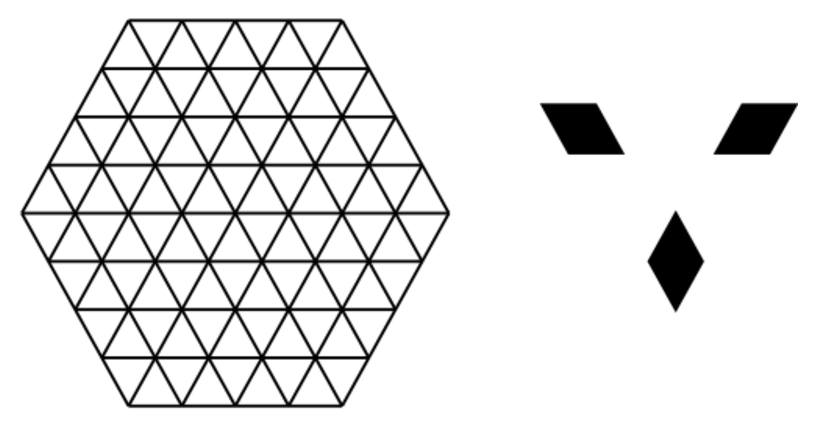
\includegraphics[scale=0.55]{Figs/Geometry/hex}
\end{figure}

\subsection*{Замощение ромбами}% (RHOMBUS TILING)
\rindex{Замощение ромбами} 

Давайте попробуем ещё раз, но плитки будут больше и больше будет число сторон.

Рассмотрим $\binom n2$ различных ромбов, образованных парами непараллельных сторон правильного $2n$-угольника.
Замостите ими $2n$-угольник, используя параллельный перенос ромбов
и докажите, что каждый ромб может использоваться ровно один раз в любом таком замощении.

\subsection*{Векторы на многограннике}% (VECTORS ON A POLYHEDRON)
\rindex{Векторы на многограннике}

Каждой грани многогранника соответствует вектор, перпендикулярный грани, направленный вовне, и имеющий длину, равную площади грани.
Докажите, что сумма этих векторов равна нулю.

\subsection*{Три окружности}% (THREE CIRCLES)
\rindex{Три окружности}

Назовём фокусом двух окружностей точку пересечения двух прямых, каждая из которых является касательной к обеим окружностям, но не проходит между ними.
Таким образом, три окружности различных радиусов (не лежащих в друг друге)
определяют три фокуса.
Докажите, что эти три фокуса лежат на одной прямой.

\begin{figure}[h!]
\centering
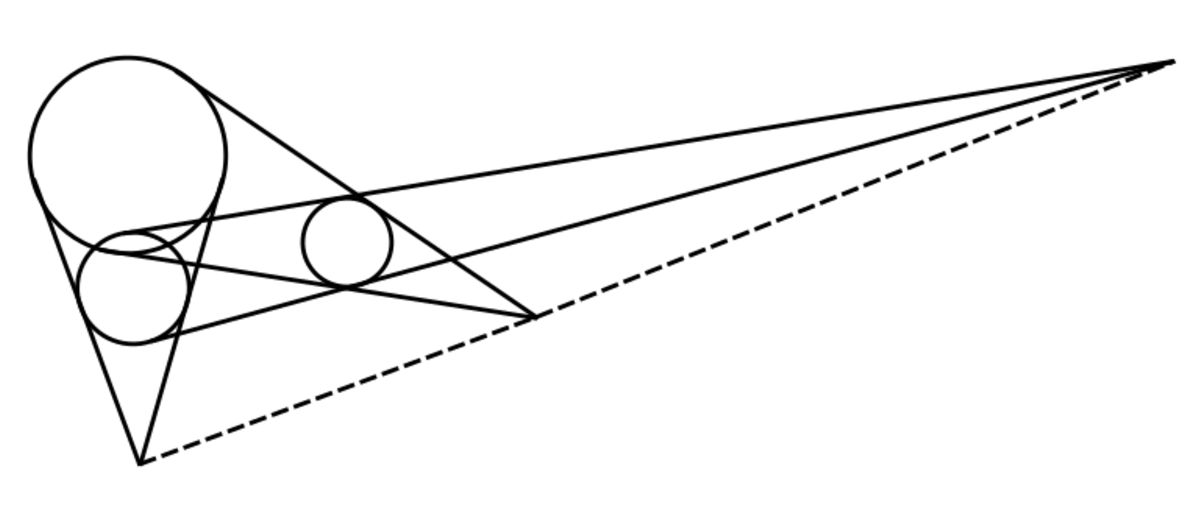
\includegraphics[scale=0.5]{Figs/Geometry/foci}
\end{figure} 

\subsection*{Сфера и четырёхугольник}% (SPHERE AND QUADRIATERAL)
\rindex{Сфера и четырёхугольник}

Пространственный четырёхугольник касается всеми сторонами сферы.
Докажите, что все точки касания лежат в одной плоскости.

\medskip

Последняя задача является небольшой экскурсией в топологию и иерархию бесконечностей.

\subsection*{Восьмёрки на плоскости}% (FIGURES 8S IN THE PLANE)
\rindex{Восьмёрки на плоскости}

Сколько непересекающихся топологических «восьмёрок» можно нарисовать на плоскости?

\begin{figure}[h!]
\centering
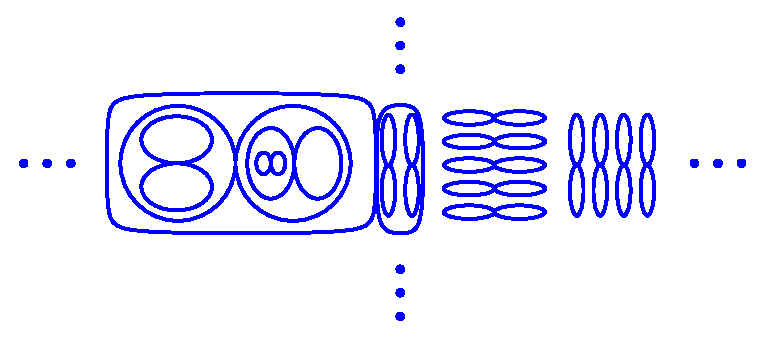
\includegraphics[scale=0.5]{Figs/Geometry/eights}
\end{figure} 
